\hiddensubsection{Prototypes With Focus on Reminders}
\label{app:HPIPrototypes}

\hiddensubsubsection{Trunk Shelf}
\label{sec:trunkshelf}

The Trunk Shelf is the result of expanding our imagined world of implementation to future and impossible scenarios. The Trunk Shelf is the idea that every apartment is built in a way that enables it to automatically move parts of the apartment into the trunk of the car and back. More specifically, the Trunk Shelf is a shelf with different compartments which resemble storage space in the car (glove box, middle compartment, trunk). Objects stored in this shelf auto-magically get transferred to the car to the corresponding space when users are inside the car and back when they are arriving at their homes (see also Figure \ref{fig:trunkshelf}. It is based on two hypotheses:

\begin{enumerate}
    \item People see a benefit in packing their luggage at home.
    \item People see a benefit in carrying part of their home/car with them.
\end{enumerate}

\begin{figure}[ht]
\centering
	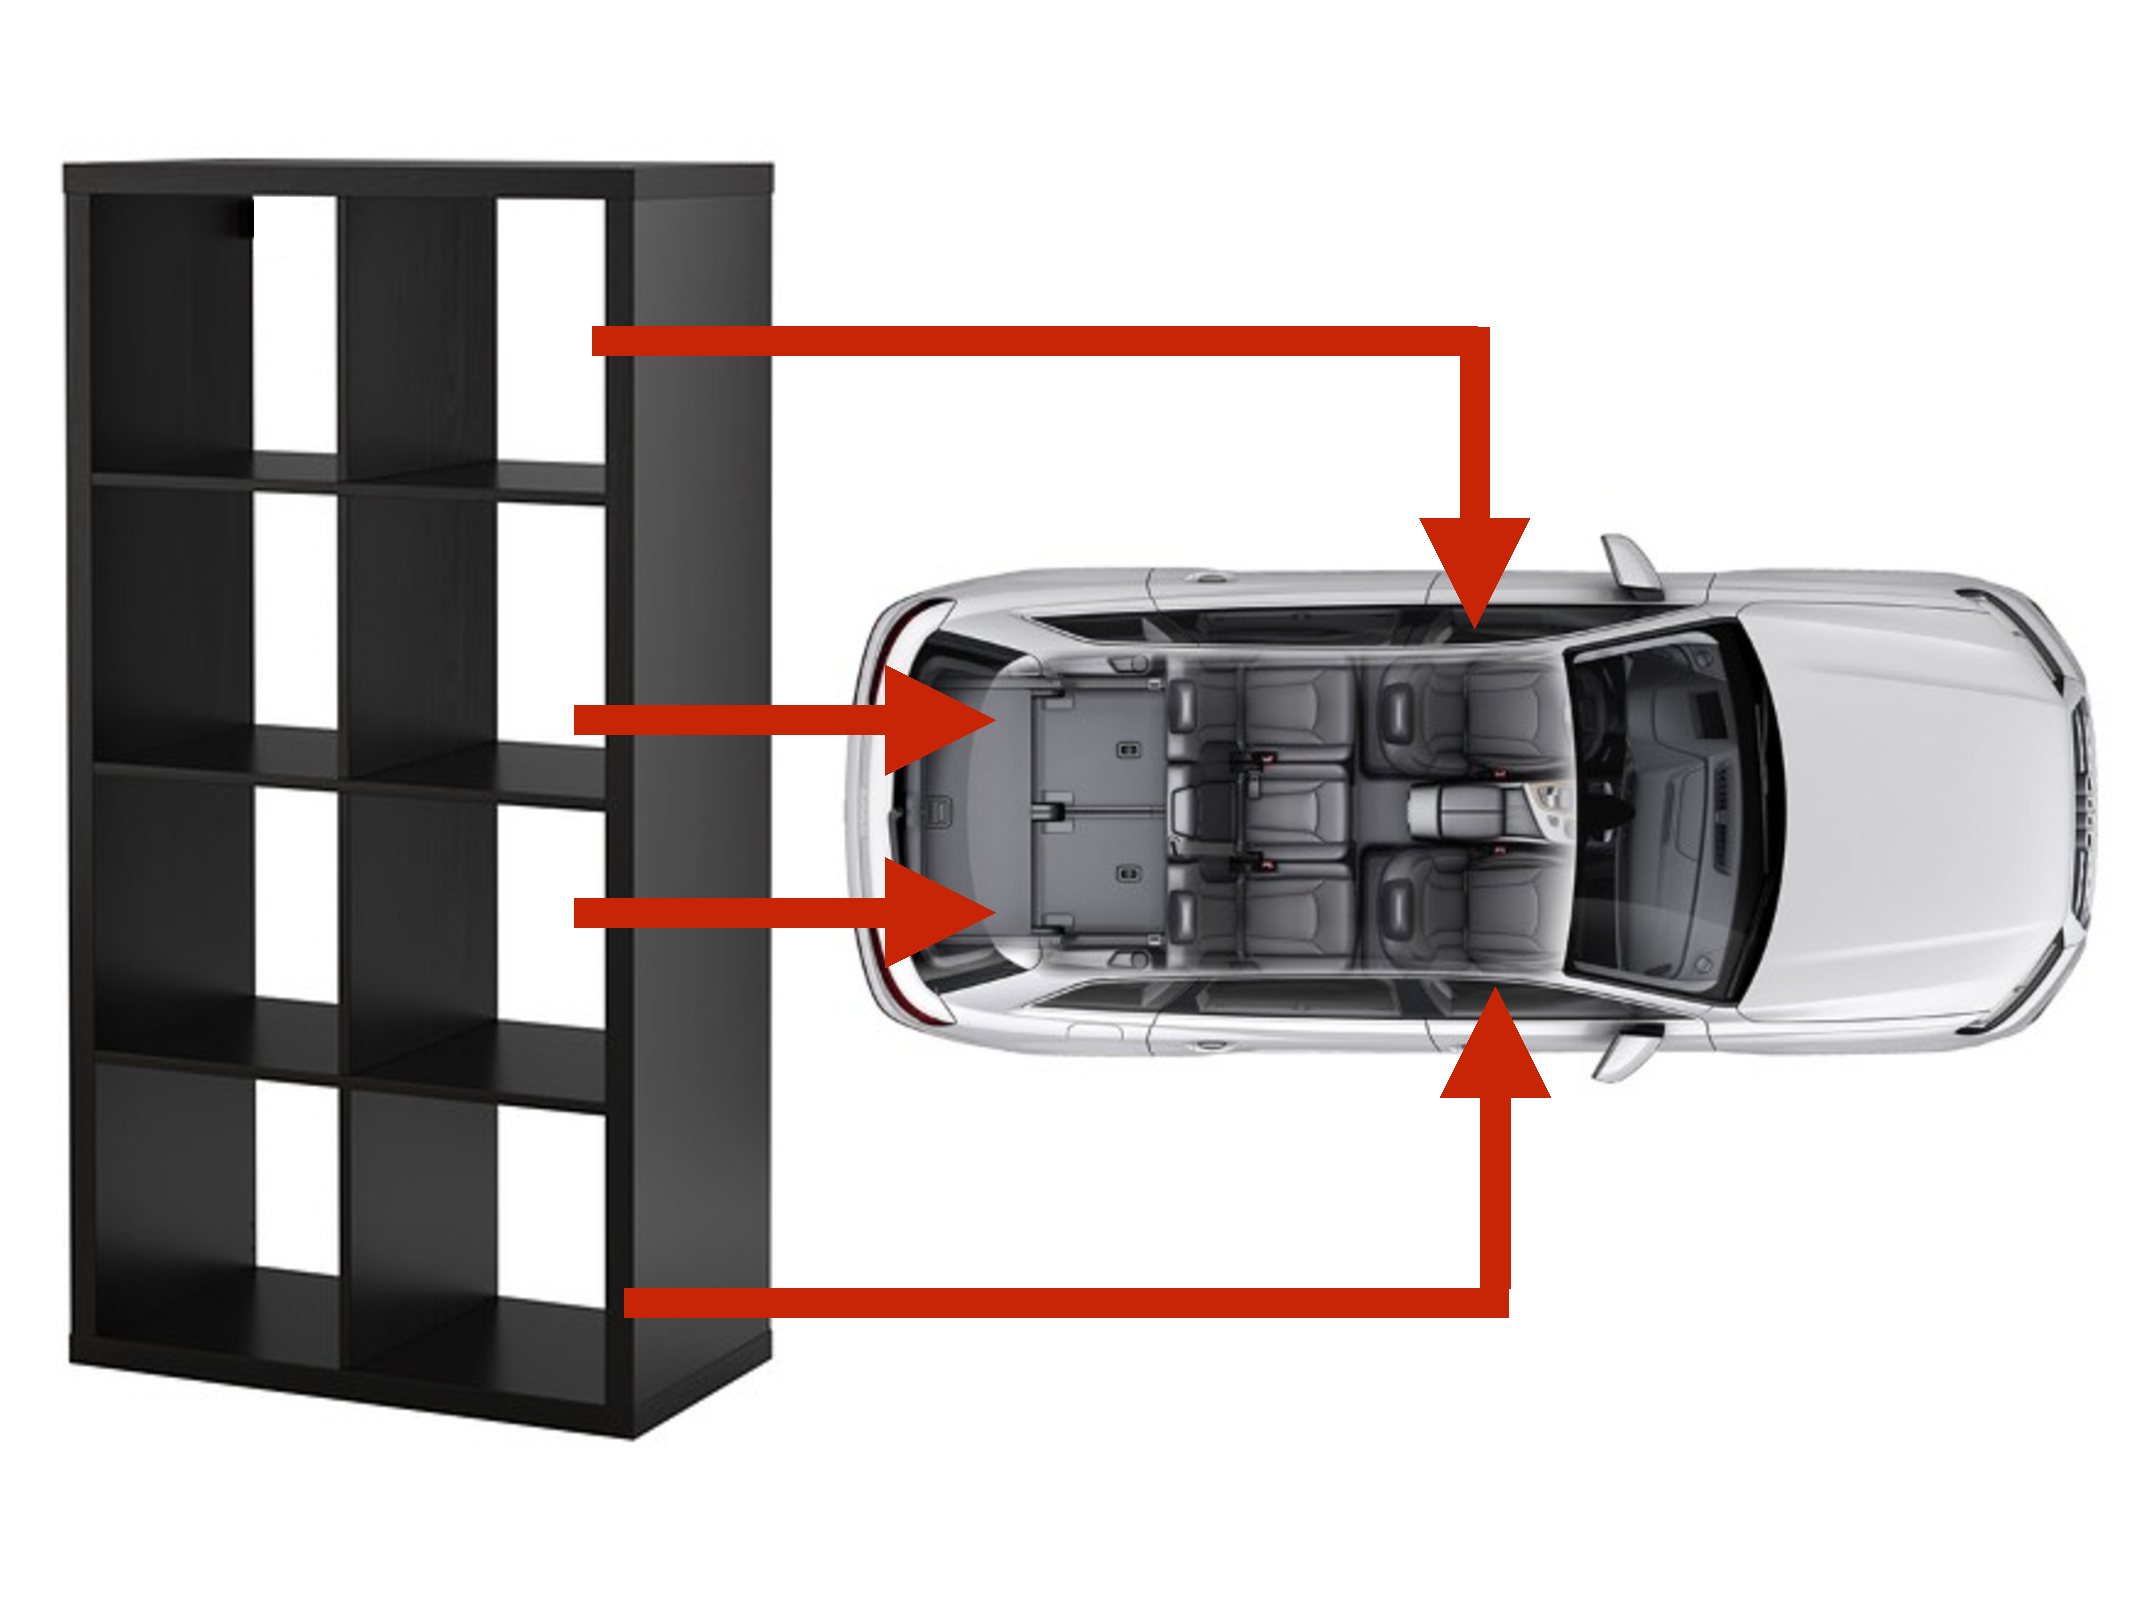
\includegraphics[keepaspectratio, width=\textwidth]{Figures/Prototypes/DarkHorse/TrunkShelf}
	\caption[appears in list of figures]{The Trunk Shelf concept. An item placed inside the Trunk Shelf is transferred auto-magically to a corresponding compartment inside the car.\protect\footnotemark}
	\label{fig:trunkshelf}
\end{figure}

\footnotetext{Sources: Audi Q7 from above: \url{http://www.audi.de/de/brand/de/neuwagen/q7/q7/layer/galerie.html}\\
\indent{} IKEA Kallax shelving unit: \url{http://www.ikea.com/us/en/images/products/kallax-shelving-unit-brown__0243982_PE383241_S4.JPG}}

During testing this idea, we found out that our testers reflected our thinking behind our first hypothesis but didn't care much for our second hypothesis. We also learned that while people find it useful to be able to pack their luggage at home, they wished they would be supported in that by reminding them about things they had forgotten.

Other learnings from this prototype were:

\begin{itemize}
    \item Shelf has to exactly map to the car (size­and functionality­wise), especially for bigger trips
    \item Time for teleport would be essential
    \item If the whole shelf could teleport to other places too (eg hotel), it would be even greater
    \item Security is very important (What happens if the car gets stolen / broken into?)
    \item Reaction to usage in daily life mixed
    \item ``Need'': I wouldn’t forget things in the car/at home so often (documents, phone, drinks), it would help me to keep an overview; it would be awesome for grocery shopping
    \item ``Don't need'': Small things in the car do not change often, I would not need the shelf for that and for big things it is too small; I don’t prepare leaving at home; it’s only useful if the car is parked far away
\end{itemize}

\hiddensubsubsection{Detachable Trunk}

The main insights that we gained during the testing of the Trunk Shelf prototype (as described in previous section \ref{sec:trunkshelf}) involve shopping experiences. We found that carrying groceries from the shop to the car and then from the car to the home is a major pain point for our testers. At the same time they had trouble remembering important things to pack when leaving home.

To cater for these needs we proposed a autonomous, portable trunk. A part of the trunk would be detachable and could autonomously follow the user. The trolley-like device could be used flexibly to remove the necessity to carry heavy items like groceries to and from the car. The device would also have a reminder display, showing for example a shopping list.

\begin{figure}[ht]
\centering
	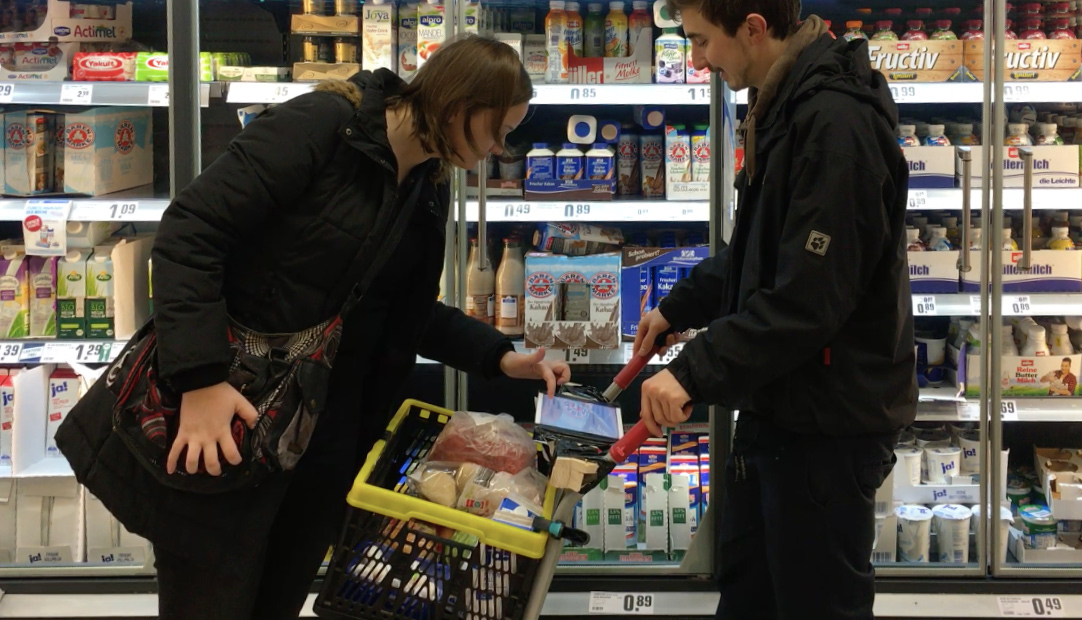
\includegraphics[keepaspectratio, width=\textwidth]{Figures/Prototypes/Funky/shopping_cart}
	\caption{The Funky prototype being used by one of our testers.}
	\label{fig:shopping_cart}
\end{figure}

Figure \ref{fig:shopping_cart} displays our prototype. We attached a foldable box to a hand truck. We mocked the autonomous property of the trolley by pushing it manually, following our test subjects. An iPad is attached to show a reminder list.

Figure \ref{fig:demtruk} shows a product of the KE Group, the dem-truk. It visualizes how we imagine parts of the folding mechanism. However we imagine a more sophisticated way without involving the several manual steps but rather harness the push or pull movement when loading or unloading the device to fold the legs.

\begin{figure}[ht]
\centering
	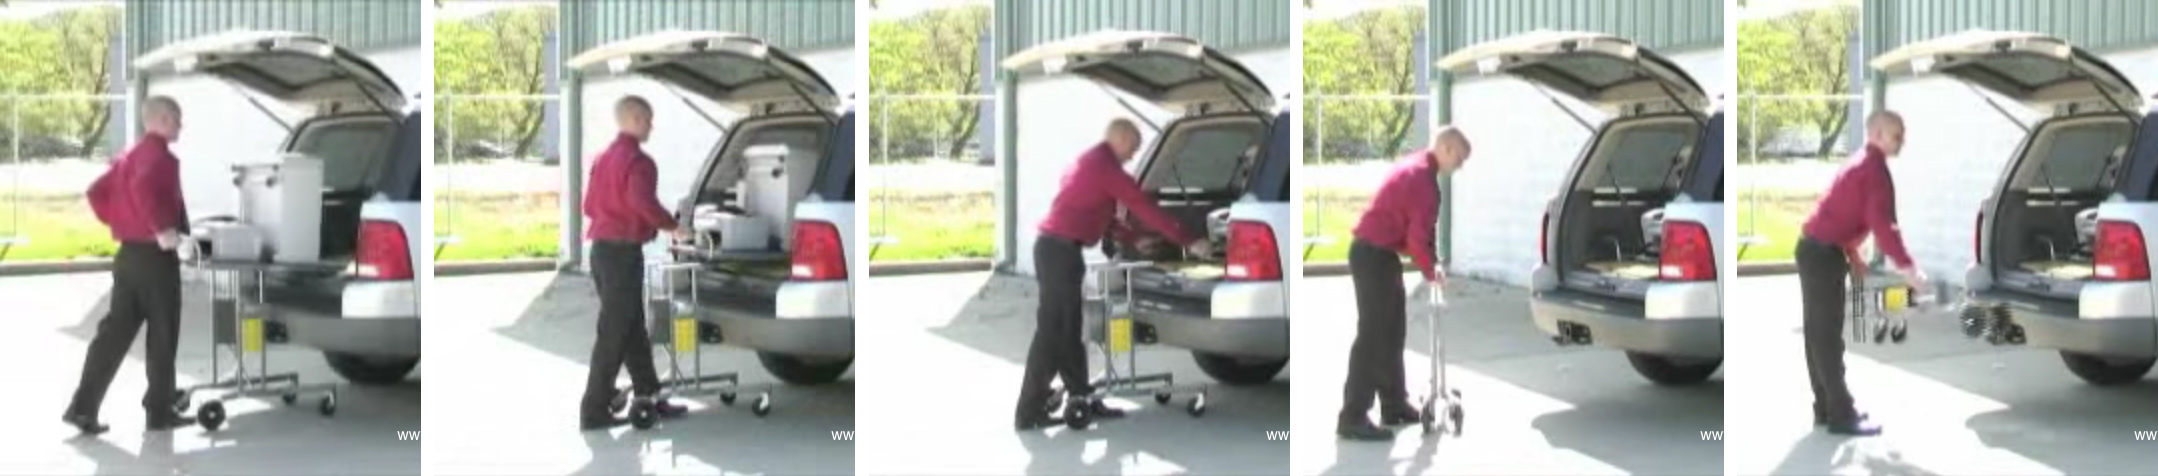
\includegraphics[keepaspectratio, width=\textwidth]{Figures/Prototypes/Funky/demtruk}
	\caption[The dem-truk trolley.]{The dem-truk folding pallet trolley in use to load a car.\protect\footnotemark}
	\label{fig:demtruk}
\end{figure}

\footnotetext{Taken from \url{https://www.youtube.com/watch?v=tqlNyYGxJgI} on March 15th 2016}

We conducted two test sessions with several users each and iterated in between. During our first session we noticed that we put too much focus on the shopping experience. It did not convey our idea of a general, multi-purpose part of the trunk following the test subject but instead our testers thought we want to learn about the supermarket shopping. In addition the concept of the trolley automatically folding into the trunk was hard to grasp since the hand truck was quite massive and non-foldable.

The second iteration improved on the aforementioned issues by having a lighter, completely foldable prototype and putting the focus onto the transition from the testers homes to the car and after the shopping from the car back into their homes. 

An important takeaway from our testing was if we would build a device that moves from the home to the car and back, we have to ensure that it does not bring dirt into the apartment. Our testers were very concerned about this aspect. 
Furthermore users do not want to give away storage space of their car, so the trolley would have to very compact when loaded into the trunk. In general there was some discussion about the size of the device - our insight is that it would have to be very flexible to be appealing to our testers.
The trust of users into an autonomously following trolley is an issue. The technology must be near perfect, our test subjects would not use it if it gets stuck from time to time.
We noted for our later prototypes that we need to refocus on subjects closer related to the homes of the users, even though we also acquired quite some knowledge about the shopping experience itself: there is a big need for in-door supermarket navigation and the time at check-out is stressful for the users.
